\section{GROUP THEORY}
\subsection{Group Definition}
A \textbf{Group} G, is a set with a rule for assigning to every (ordered) pair of
elements, a third element, satisfying:

1. If f, g $\epsilon$ G then h = fg $\epsilon$ G. \\
2. Associativity: $\forall$ f, g, h $\epsilon$ G, f(gh) = (fg)h. \\
3. Existence of identity element: $\forall$ f $\epsilon$ G $\exists$ \textit{e} s.t. \textit{e}f = f\textit{e} = f. \\
4. Existence of inverse element: $\forall$ f $\epsilon$ G $\exists$ f $^{-1}$ s.t. f f$^{-1}$ = f$^{-1}$f = \textit{e}.
\begin{figure}[h]
    \centering
    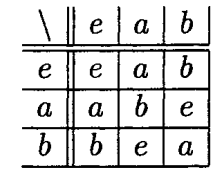
\includegraphics[width=0.3\textwidth]{figures/z3-group.png}
    \caption{Z$_3$ group multiplication table. (Every row and column
    of the multiplication table contains each element of the group exactly once.
    This must be the case because the inverse exists.)}
\end{figure}

A group G is \textbf{finite} if it has a finite number of elements. Otherwise it is \textbf{infinite}.
The number of elements in a finite group G is called the \textbf{order} of G. For eg: Z$_3$, the cyclic group of order 3.

An \textbf{Abelian group} G in one in which the multiplication law is commutative i.e.
g$_1$g$_2$ = g$_2$g$_1$. And the one which doesn't follows commutation is called \textbf{non-Abelian group}.

A \textbf{Representation} of a group G is a mapping D of the elements of G onto a set of
linear operators with the following properties:

1. D(\textit{e}) = 1, where 1 is the identity operator in the space on which
the linear operators act. \\
2. D(g$_1$)D(g$_2$) = D(g$_1$g$_2$) i.e. the group multiplication law 
is mapped onto the natural multiplication in the linear space on which the linear operators act.

For eg: representation of Z$_3$ is,
\begin{equation}
    D(e) = 1, \hspace{1cm} D(a) = e^{2\pi i/3}, \hspace{1cm} D(b) = e^{4\pi i/3}
\end{equation}
another representation of Z$_3$ can be directly constructed from the multiplication table as,
\begin{equation}
    D(e) = \begin{pmatrix}
        1 & 0 & 0 \\ 
        0 & 1 & 0 \\ 
        0 & 0 & 1 \\ 
   \end{pmatrix}, \hspace{1cm} 
   D(a) = \begin{pmatrix}
        0 & 0 & 1 \\ 
        1 & 0 & 0 \\ 
        0 & 1 & 0 \\ 
   \end{pmatrix}, \hspace{1cm} 
   D(b) = \begin{pmatrix}
        0 & 1 & 0 \\ 
        0 & 1 & 1 \\ 
        1 & 0 & 0 \\ 
\end{pmatrix},
\end{equation}

By taking the group elements themselves to form an orthonormal basis for a vector space, 
$|e \rangle$, $|a\rangle$, and $|b\rangle$ we can also define \textbf{regular representation} as,
\begin{equation}
    D(g_1)|g_2\rangle = |g_1g_2\rangle
    \label{eqn:representation}
\end{equation}

The \textbf{dimension of a representation} is the dimension of the space on which
it acts and the dimension of the regular representation is the order of the group. The representation of Z$_3$ is 1 dimensional.
For any finite group, we can define a vector space in which the basis vectors are labeled by the group elements.
Then equation \ref{eqn:representation} defines the regular representation.








\subsection{Lie Group}
\href{https://aimath.org/E8/liegroup.html#:~:text=Lie%20groups%20lie%20at%20the,are%20examples%20of%20smooth%20manifolds.}{Lie group}
The definition above is easy to use, but it is not defined for Lie groups that are not matrix groups,  and it is not clear that the \href{https://en.wikipedia.org/wiki/Lie_group}{exponential map}
of a Lie group does not depend on its representation as a matrix group. 
We can solve both problems using a more abstract definition of the exponential map that works for all Lie groups.


\newpage